\documentclass[11pt]{article}
\pagenumbering{gobble}
\setlength\parindent{0pt}

\usepackage{graphicx}
\usepackage{apacite}

\begin{document}

\section*{Introduction}

Physical activity (PA) has long been established as one of the main contributors to prevent chronic diseases and promote health \cite{Kaminsky_2014, Warburton_2017}. Evidence shows that lack of PA leads to an increased risk of cardiovascular disease, diabetes, hypertension, osteoporosis, several types of cancer and a higher mortality rate \cite{Guthold_2018, Lee_2012, Shiroma_2014}. Given the relevant relationship between PA and health, there is an increasing need of accurate and reliable methods of PA assessment on daily life \cite{Montoye_2000, Plasqui_2013, Strath_2013}. These methods can be either subjective, such as questionnaires, or objective, as direct observation and wearable devices \cite{Strath_2013, Troiano_2005}. \\

The most commonly used wearable devices to assess PA are accelerometers \cite{Strath_2013}, described as equipments that detect the body movement accelerations in one to three orthogonal planes (anteroposterior, mediolateral, and vertical) \cite{Chen_2005}. The accelerometers output can be either raw acceleration, usually expressed as gravitational acceleration units (\textit{g}), or activity counts, which are processed data derived from the raw acceleration and are based on manufacturer-specific algorithm \cite{Chen_2005, Basset_2012, Troiano_2014}. In both cases, the accelerometer output needs to be translated into more biologically meaningful information through a calibration process \cite{Matthews_2005}. \\

Currently, most calibration studies use the accelerometer output to relate to energy expenditure (EE) and PA intensity levels \cite{Migueles_2017, Mendes_2018} but they can be also used to estimate biomechanical parameters, such as ground reaction forces (GRF) \cite{Neugebauer_2014, Fortune_2014}, to evaluate standing balance \cite{Mayagoitia_2002}, to detect the type of PA being performed \cite{Bonomi_2009, Zhang_2012}, among others. Apart from the standard measure against which the accelerometer output needs to be compared	, calibration studies must carefully define the sample characteristics, PA protocols and statistical approaches, as these aspects can greatly influence the study internal and external validity \cite{Basset_2012, Welk_2005}. This led to the emergence of several different calibration studies in the literature with distinct methods to predict a given outcome variable \cite{Mendes_2018, Matthews_2018}. \\

This current review aims to describe the literature regarding the use of accelerometers to measure EE, classify physical activity intensities and estimate GRF, as well as issues about calibration and validation studies of these wearable monitors. 

\section*{Accelerometers}

As said before, accelerometers are wearable devices used to measure PA related variables \cite{Chen_2005}. The first portable accelerometer was developed in the 1980s \cite{Wong_1981, Montoye_1983} and with the many technological advances since then, the use of such devices in research is ever growing, with a major increase in the number of published articles mentioning PA or exercise and accelerometers since the early 2000s (Figure \ref{art_year}).

\begin{figure}[h!]
	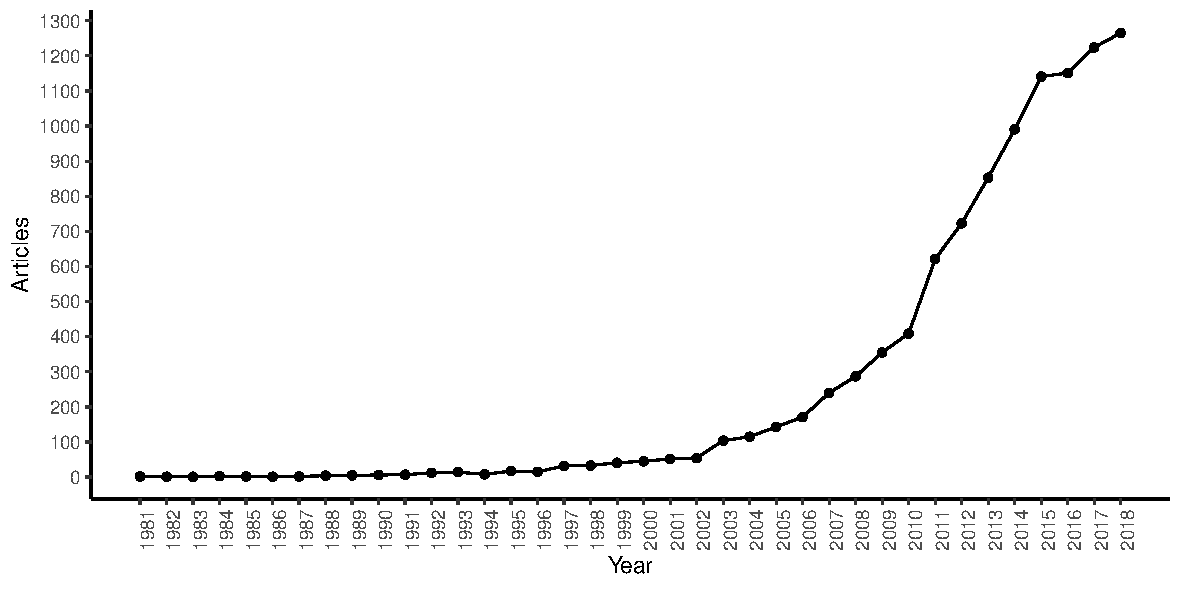
\includegraphics[width=\linewidth]{../figs/fig1.tiff}
	\caption{Articles published by year with search terms ``exercise or physical activity'' and ``accelerometer or accelerometry'', Scopus.com, accessed 15 April 2019.}
	\label{art_year}
\end{figure}

From a technical standpoint, the working principle of most accelerometers is based on a sensing element, the seismic mass, and a piezoelectric element. When this system suffers an acceleration, the seismic mass causes a deformation in the piezoelectrical element, generating an output voltage signal proportional to the applied acceleration \cite{Chen_2005, Yang_2010}. The rate by which this data is acquired is determined by the sampling frequency of the device, making it responsive not only to the acceleration intensity, but to its frequency \cite{Mathie_2004}. The signal is then filtered and processed before being digitally stored by the equipment \cite{Chen_2005}. \\

As an objective method to measure PA, accelerometers offer some advantages over subjective methods, such as questionnaires and PA diaries. They are capable of long data collection with low subject burden \cite{Chen_2012, Strath_2013}, are more accurate than questionnaires to measure PA and sedentary behaviour \cite{Celis-Morales_2012, Matthews_2018} and can measure the full spectrum of daily activities, providing detailed intensity, frequency and duration data \cite{Matthews_2018, Strath_2013}. \\

On the other hand, accelerometer devices also present some weaknesses. They cannot account for some activities, such as cycling, climbing stairs, weight-lifting and upper-body activities when worn at hip or lower back \cite{Strath_2013}. Also, different manufacturers have distinct algorithms to compute activity counts, making these data not comparable between devices \cite{Plasqui_2013}. And there is still no consensus on where to place accelerometers on the body, and how to process the data \cite{Troiano_2014}. \\

Some decisions need to be made in order to conduct a research utilising accelerometers, such as the device sampling frequency, body placement in which to wear it, and which accelerometer output to use (either activity counts or raw acceleration). To assure that all human movements are correctly captured by the monitor, the sampling frequency must be at least twice the highest movement frequency, accordingly to the Nyquist criterion \cite{Chen_2012}. The first accelerometry studies utilised a sampling frequency of 30 Hz, which was the limit of most equipments at that time, but nowadays the recommendation ranges from 90 to 100 Hz \cite{Migueles_2017}. \\

As to the body placement in which to wear the accelerometers, the waist is the most common as it is the closest to the body center of mass \cite{Chen_2005, Mendes_2018}. Other placements are the lower back \cite{Brandes_2012}, wrist \cite{Hildebrand_2017}, ankle \cite{Fortune_2014} and thigh \cite{Montoye_2016}. Among these body placements, wrist has been gaining popularity on the past few years, most due to its increase in prediction accuracy with  some recent studies \cite{Phillips_2013, Hildebrand_2017} and its improved compliance compared with waist placement. These facts made the United States National Health and Nutrition Examination Survey (NHANES) change from waist to wrist placement in the 2011-2012 and 2013-2014 cycles \cite{Troiano_2014}. \\

Early studies on accelerometry utilised the activity counts as they were the only available technology at that time. Despite presenting moderate to high correlations with measured EE \cite{Nichols_1999, Freedson_1998} and GRF \cite{Janz_2003}, activity counts calculation depends on proprietary algorithms that vary among manufacturers, causing different accelerometers to produce different count values even when measuring the same accelerations \cite{Chen_2012, Plasqui_2013}. \\

Recent technological advances have enabled to collect and store raw acceleration data at high frequencies, eliminating the need to summarise them in activity counts \cite{Bakrania_2016}. The use of raw acceleration entails some advantages, as the ability to extract time-domain and frequency-domain features from the data, allowing to apply more advanced statistical and computational techniques in the calibration process \cite{John_2013}. It can also enhance comparability among accelerometers from different manufacturers \cite{Mendes_2018, Rowlands_2016}. \\

With these modern technologies and the recent endorsement to the use of raw acceleration \cite{Freedson_2012}, several metrics based on raw acceleration have been developed, as the euclidean norm minus one (ENMO) \cite{vanHees_2013}, the mean amplitude deviation (MAD) \cite{Vaha-Ypya_2015} and the activity index (AI) \cite{Bai_2016}. The use of these new metrics also complies with the recommendations for more transparency \cite{Intille_2012}, since they are nonproprietary metrics, with known properties and can be computed using open-source software.

\bibliography{bibliography}
\bibliographystyle{apacite}

\end{document}